This chapter is dedicated to introducing the neutron transport equation and numerical methods commonly used to solve it.  First, the transport equation will be introduced and all its terms defined.  Some common approximations that are needed to make the transport equation more practically solvable will also be introduced.  Second, numerical methods will be discussed and, when appropriate, derived from the transport equation.  The theory is covered in detail in a variety of textbooks \cite{NEHandbook-PrinciplesOfTransport}, and other texts discuss numerical methods to solve the transport equation \cite{AppliedReactorPhysics}.  This chapter will not attempt to reiterate all that can be found in these references, but rather to highlight the theory and methods which are relevant to this work.

\section{Boltzmann Equation}

The time-dependent Boltzmann equation for neutron transport is shown below:
\begin{subequations}\label{e:boltzmann}
\begin{dmath}
{\frac{1}{v} \frac{\partial \varphi}{\partial t} + 
\bm \Omega \cdot \bm \nabla \varphi + \Sigma_t\left(\bm x,E,t\right)\varphi\left(\bm x,E,\bm \Omega,t\right)} = {\frac{1}{4\pi}\intop_0^{\infty} \intop_{4\pi} \Sigma_s\left(\bm x,E' \rightarrow E, \bm \Omega' \rightarrow \bm \Omega\right) \varphi\left(\bm x,E',\bm \Omega'\right) d\Omega' dE'} + {\frac{\chi_p\left(\bm x,E\right)}{4\pi} \intop_0^{\infty} \intop_{4\pi} \left(1 - \beta\left(\bm x,E'\right)\right) \nu \Sigma_f\left(\bm x,E',t\right) \varphi\left(\bm x,E',\bm \Omega',t\right) d\Omega' dE'} + {\sum_{j=1}^{N_d} \frac{\chi_{d,j}\left(\bm x,E\right)}{4\pi} \lambda_j C_j\left(\bm x,t\right)} + {Q\left(\bm x,E,\bm \Omega,t\right)}\ ,
\end{dmath}
\begin{equation}\label{e:boltzmannBC}
\varphi\left(\bm x_b, E, \bm{\Omega},t\right) = \varphi^b\left(\bm x_b, E, \bm{\Omega},t\right)\ ,\quad \bm{\Omega}\cdot \bm n_b < 0\ .
\end{equation}
\end{subequations}

Before addressing the methods used to solve Equation \ref{e:boltzmann}, we will briefly define each of the terms in the Equation \ref{e:BTEtermsTimeDerivative}.  The first term is the time derivative term, shown in , which accounts for the change in the angular flux over time in dV about $\bm x$, dE about $E$, and d$\Omega$ about $\bm\Omega$.  

\begin{equation}\label{e:BTEtermsTimeDerivative}
\frac{1}{v} \frac{\partial \varphi}{\partial t}\ .
\end{equation}

The second term (Equation \ref{e:BTEtermsStreaming} is the streaming term.  This describes neutrons with energy $E$ traveling out of the volume dV in the direction $\bm\Omega$.

\begin{equation}\label{e:BTEtermsStreaming}
\bm \Omega \cdot \bm \nabla \varphi\ .
\end{equation}

The third term is the total reaction rate (Equation \ref{e:BTEtermsTotalRR}).  This describes the total number of collisions experienced in dV by neutrons with energy $E$ and direction $\bm\Omega$.  Equations \ref{e:BTEtermsTimeDerivative}-\ref{e:BTEtermsTotalRR} together make up the total loss of neutrons.

\begin{equation}\label{e:BTEtermsTotalRR}
\Sigma_t\left(\bm x,E\right)\varphi\left(\bm x,E,\bm\Omega\right)\ .
\end{equation}

Equation \ref{e:BTEtermsScatteringSource} shows the scattering source written in a simplified form.  This is the total number of neutrons scattering into energy $E$ and direction $\bm\Omega$ from all other energies and directions $E'$ and $\bm\Omega'$ in dV.  Because scattering is symmetric around the incident angle, the scattering cross section depends only on the dot product $\bm\Omega'\cdot\bm\Omega$ rather than each of the two angles independently.

\begin{equation}\label{e:BTEtermsScatteringSource}
\intop_0^{\infty} \intop_{4\pi} \Sigma_s\left(\bm x,E' \rightarrow E, \bm \Omega' \cdot \bm \Omega\right) \varphi\left(\bm x,E',\bm \Omega'\right) d\Omega' dE'\ .
\end{equation}

Equation \ref{e:BTEtermsFissionSource} shows the prompt fission source, neutrons entering dV with energy and direction $E$ and $\bm\Omega$ directly from a fission event.  Fission is an isotropic process, so the total fission source is calculated then distributed evenly across $4\pi$.  Furthermore, the energy distribution of fission is practically independent of incident neutron energy, so the fission neutron distribution $\chi_p\left(E\right)$ can be outside the integral over energy.  A small fraction of fission neutrons are considered ``delayed,'' meaning they are emitted by the radioactive decay of a fission product.  The prompt fission source must be adjusted by the factor $\left(1-\beta\left(\bm x,E'\right)\right)$ to account for this.  Typically $\beta$ is less than 1\% and different for each fissionable isotope.

\begin{equation}\label{e:BTEtermsFissionSource}
{\frac{\chi_p\left(\bm x,E\right)}{4\pi} \intop_0^{\infty} \intop_{4\pi} \left(1 - \beta\left(\bm x,E'\right)\right) \nu \Sigma_f\left(\bm x,E',t\right) \varphi\left(\bm x,E',\bm \Omega',t\right) d\Omega' dE'}\ .
\end{equation}

Equation \ref{e:BTEtermsDelayedSource} shows the fission source due to delayed neutrons.  The precursors, fission products which emit delayed neutrons, are divided into $N_d$ groups based on the magnitude of their decay constant $\lambda_j$.  Like the prompt neutrons, delayed neutrons are isotropic and distributed in energy with some distribution $\chi_{d,j}\left(\bm x,E\right)$ based on which precursors are produced.

\begin{equation}\label{e:BTEtermsDelayedSource}
{\sum_{j=1}^{N_d} \frac{\chi_{d,j}\left(\bm x,E\right)}{4\pi} \lambda_j C_j\left(\bm x,t\right)}\ .
\end{equation}

Equation \ref{e:BTEtermsExtSource} shows external source term.  This term accounts for all neutrons entering dV with energy and direction $E$ and $\bm\Omega$ from sources other than scatter and fission.  Equation \ref{e:BTEtermsExtSource} shows the source term as a function of angle, but it is often considered to be isotropic like the fission source.

\begin{equation}\label{e:BTEtermsExtSource}
Q\left(\bm x,E,\bm\Omega\right)\ .
\end{equation}

Finally, Equation \ref{e:boltzmannBC} shows the boundary condition for the transport equation.  The dot product $\bm \Omega \cdot \bm n_b$ is between the direction of flight and the outward normal vector on the boundary of the problem.  The angular flux boundary condition defines the angular flux entering the problem domain. for the entire surface $\bm x_b$, all energies, and all times.

Many problems of interest are steady-state, allowing Equation \ref{e:boltzmann} to be simplified significantly.  The time derivative becomes 0, eliminating the term in \ref{e:BTEtermsTimeDerivative}, and the precursor concentrations are unchanging in time, allowing the fission source terms in \ref{e:BTEtermsFissionSource} and \ref{e:BTEtermsDelayedSource} to be lumped into a single term.  To ensure balance between the loss and source terms without a time derivative, the equation is reformulated as an eigenvalue equation.  The fission source is multiplied by the eigenvalue $\lambda = \frac{1}{\keff{}}$, allowing the equation to be balanced.  The cross sections can then be adjusted until $\lambda = 1$ is achieved, providing a physically meaningful steady-state solution to the equation.  The steady-state form of the Boltzmann equation is shown below:

\begin{subequations}\label{e:ssboltzmann}
\begin{dmath}
{\bm \Omega \cdot \bm \nabla \varphi + \Sigma_t\left(\bm x,E\right)\varphi\left(\bm x,E,\bm \Omega\right) = \frac{1}{4\pi}\intop_0^{\infty} \intop_{4\pi} \Sigma_s\left(\bm x,E' \rightarrow E, \bm \Omega' \rightarrow \bm \Omega\right) \varphi\left(\bm x,E',\bm \Omega'\right) d\Omega' dE'} + {\frac{1}{\keff{}}\frac{\chi\left(E\right)}{4\pi} \intop_0^{\infty} \intop_{4\pi} \nu \Sigma_f\left(\bm x,E'\right) \varphi\left(\bm x,E',\bm \Omega'\right) d\Omega' dE'}\ ,
\end{dmath}
\begin{equation}\label{e:ssboltzmannBC}
\varphi\left(\bm x_b, E, \bm{\Omega}\right) = \varphi^b\left(\bm x_b, E, \bm{\Omega}\right)\ ,\quad \bm{\Omega}\cdot \bm n_b < 0\ .
\end{equation}
\end{subequations}

\subsection{Multigroup Approximation}

One important approximation that is commonly made to the transport equation is the multi-group approximation.  To make this approximation, an appropriate energy range for the problem of interest is selected.  As illustrated in Figure \ref{f:multigroup}, this energy range is divided up into $G$ energy groups, with each group going from $E_g$ up to $E_{g-1}$.  For light-water reactor problems, it is common to select 0 eV for $E_N$ and 20 MeV for $E_0$.

\begin{figure}[h]
    \centering
    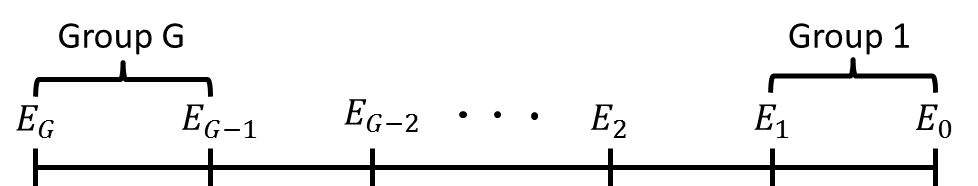
\includegraphics[width=0.8\textwidth]{MGillustration.png}
    \caption{Illustration of the multigroup discretization scheme}\label{f:multigroup}
\end{figure}

We first define the multi-group flux, cross sections, and chi distribution in Equations \ref{e:multigroupDefinitions}.  These definitions ensure that the total reaction rates are preserved in each energy interval $g$.
\begin{subequations}\label{e:multigroupDefinitions}
\begin{equation}\label{e:multigroupangflux}
\varphi_g\left(\bm x,\bm \Omega\right)= \intop_{E_n}^{E_{n-1}} \varphi\left(\bm x,E,\bm\Omega\right) dE\ ,
\end{equation}
\begin{dmath}\label{e:multigroupXS}
{\Sigma_{x,g}\left(\bm x,\bm \Omega\right) \varphi_g\left(\bm x,\bm \Omega\right) =  \intop_{E_n}^{E_{n-1}} \varphi\left(\bm x, E, \bm \Omega\right) \Sigma_x\left(\bm x, E, \bm \Omega\right) dE} \Rightarrow {\Sigma_x,g\left(\bm x, \bm \Omega\right) = \frac{\intop_{E_n}^{E_{n-1}} \varphi\left(\bm x, E, \bm \Omega\right) \Sigma_x\left(\bm x, E, \bm \Omega\right) dE}{\intop_{E_n}^{E_{n-1}} \varphi\left(\bm x, E, \bm \Omega\right) dE}}\ .
\end{dmath}
\end{subequations}
Using the definitions above, Equation \ref{e:ssboltzmann} can be operated on by 
$\intop_{E_n}^{E_{n-1}}\left(\cdot\right)dE$ to obtain the multi-group 
transport Equation \ref{e:multigroupboltzmann}.
\begin{subequations}\label{e:multigroupboltzmann}
\begin{dmath}
{\bm \Omega \cdot \bm \nabla \varphi_g + \Sigma_{t,g}\left(\bm x\right)\varphi_g\left(\bm x,\bm \Omega\right) = \frac{1}{4\pi}\sum_{g'=1}^G \intop_{4\pi} \Sigma_{s,g'\rightarrow g}\left(\bm x,\bm \Omega' \rightarrow \bm \Omega\right) \varphi_{g'}\left(\bm x,\bm \Omega'\right) d\Omega'} + {\frac{1}{\keff{}}\frac{\chi_g}{4\pi} \sum_{g'=1}^{G} \intop_{4\pi} \nu \Sigma_{f,g'}\left(\bm x\right) \varphi_{g'}\left(\bm x,\bm \Omega'\right)d\Omega'}\ ,
\end{dmath}
\begin{equation}\label{e:multigroupboltzmannBC}
\varphi_g\left(\bm x_b, \bm{\Omega}\right) = \intop_{E_n}^{E_{n-1}} \varphi^b\left(\bm x_b, E, \bm{\Omega}\right)dE\ ,\quad \bm{\Omega}\cdot \bm n_b < 0\ .
\end{equation}
\end{subequations}

\subsection{Discrete Ordinates Approximation}

In addition to energy discretization, it is also useful to discretize the transport equation in angle.  The angular variable $\bm\Omega$ is made up of a polar angle ($\mu$) and an azimuthal angle ($\alpha$), where the polar angle is defined with respect to the z-axis and the azimuthal angle is defined with respect to the x-axis in the x-y plane.  Both angles can be discretized as follows:
\begin{subequations}
\begin{align}
\bm\Omega &= \cos\left(\alpha\right)\sqrt{1-\mu^2}\bm i + \sin\left(\alpha\right)\sqrt{1-\mu^2}\bm j + \mu\bm k \\
\Rightarrow \bm\Omega_n &= \cos\left(\alpha_n\right)\sqrt{1-\mu_n^2}\bm i + \sin\left(\alpha_n\right)\sqrt{1-\mu_n^2}\bm j + \mu_n\bm k\ .
\end{align}
\end{subequations}

For each $\bm\Omega_n$, there is an associated weight $w_n$.  These weights and angles together make up an angular quadrature set which simplifies the integrals in Equations \ref{e:quadratureIntegrals}.
\begin{subequations}\label{e:quadratureIntegrals}
\begin{equation}
\intop d\Omega = \sum_{n=1}^N w_n = 4\pi\ ,
\end{equation}
\begin{equation}
\intop \bm\Omega d\Omega = \sum_{n=1}^N \bm\Omega_n w_n = 0\ ,
\end{equation}
\begin{equation}
\intop_{4\pi} f\left(\bm\Omega\right)d\Omega \approx \sum_{n=1}^N f_n w_n\ .
\end{equation}
\end{subequations}
Applying this discretization to the multi-group transport Equation \ref{e:multigroupboltzmann}, we obtain the following discrete ordinates (S$_N$) equations:
\begin{subequations}\label{e:SnBoltzmann}
\begin{dmath}
\bm\Omega_n\cdot\bm\nabla\varphi_{g,n} + \Sigma_{t,g}\left(\bm x\right)\varphi_{g,n}\left(\bm x\right) = {\frac{1}{4\pi}\sum_{g'=1}^G \sum_{n'=1}^N \Sigma_{g'\rightarrow g,n'\rightarrow n}\left(\bm x\right)\varphi_{g',n'}\left(\bm x\right) w_{n'}} + {\frac{1}{\keff{}}\frac{\chi_g}{4\pi} \sum_{g'=1}^G \sum_{n'=1}^N \nu\Sigma_{f,g'}\left(\bm x\right)\varphi_{g',n'}\left(\bm x\right) w_{n'}}\ ,
\end{dmath}
\begin{equation}
\varphi_{g,n}\left(\bm x_b\right) = \varphi_{g}^b\left(\bm x_b,\bm{\Omega}_n\right)\ ,\quad \bm{\Omega}_n\cdot \bm n_b < 0\ .
\end{equation}
\end{subequations}

\subsection{Scattering Approximations}

One of the biggest challenges to solving the transport equation is angle dependence of the scattering cross sections and angular flux.  To simplify the scattering cross sections, there are two different types of approximations that can be made in MPACT.

\subsubsection{P\texorpdfstring{$_N$}{N} Scattering}

The first scattering approximation that can be made is P$_N$ scattering.  To make this approximation, the $\bm\Omega'\cdot\bm\Omega$ is rewritten as a single angular variable $\mu_s$, the cosine between the incoming and outgoing scattering angles.  The scattering cross section can then be expanded in terms of Legendre polynomials, defined by Equations \ref{e:LegendrePolynomials}.
\begin{subequations}\label{e:LegendrePolynomials}
\begin{equation}
P_{n+1}\left(\mu_s\right) = \frac{\left(2n+1\right)\mu_s P_n\left(\bm 
    \mu_s\right) - 
    nP_{n-1}\left(\mu_s\right)}{n+1}\ ,
\end{equation}
\begin{equation}
P_0\left(\mu_s\right) = 1\ ,
\end{equation}
\begin{equation}
P_1\left(\mu_s\right) = \mu_s\ ,
\end{equation}
\begin{equation}
\intop_{-1}^1 P_n\left(\mu_s\right) P_m\left(\mu_s\right) d\mu_s = 
\frac{2}{2n+1}\delta_{n,m}\ .
\end{equation}
\end{subequations}

Equations \ref{e:PnScatteringExpansion} show the expansion of the scattering cross section using Legendre polynomials.  Using more terms in the expansion improves the accuracy.  For most reactor problems, $N \le 3$ is sufficient.  Problems such as shielding and others may require many more terms to be kept to obtain sufficient accuracy.
\begin{subequations}\label{e:PnScatteringExpansion}
\begin{equation}
\Sigma_s\left(\bm x,\mu_s\right) = \sum_{n=0}^N \frac{2n+1}{4\pi} P_n\left(\mu_s\right) \Sigma_{sn}\left(\bm x\right)\ ,
\end{equation}
\begin{equation}
\Sigma_{s,n}\left(\bm x\right) = 2\pi\intop_{-1}^1 \Sigma_s\left(\bm x,\mu_s\right) P_n\left(\mu_s\right) d\mu_s\ .
\end{equation}
\end{subequations} 

\subsubsection{Transport Correction}\label{sss:TCP0}

A second simplification of the scattering source that can be used is 
transport-corrected isotropic (TCP$_0$) scattering.  When using this 
approximation, the equation is solved using only the zeroth order term in 
\ref{e:PnScatteringExpansion}.  The cross section data used to develop the 
multi-group scattering cross sections is modified beforehand to still preserve 
some of the higher order scattering physics.

Currently, the MPACT code uses \cite{MPACTTheoryManual} uses a combination of 
three transport-correction methods for its TCP$_0$ scattering treatments 
\cite{StimpsonAP1000ImprovedDiffCoeffs2015,Yee2016AnAnAnalyticDerivationofTransport-CorrectedP$_0$CrossSectionsandDiffusionCoefficients}.
The Neutron Leakage Conservation (NLC) method 
\cite{Herman2013ImproveddiffusioncoefficientsgeneratedfromMonteCarlocodes} is 
used for H-1; the nTRACER in-scatter method 
\cite{RyuIncorporationofanisotropicscatteringinnTRACER} is used for B-11, C-12, 
and O-16; and the out-scatter method 
\cite{YAMAMOTO2008SimplifiedTreatmentsofAnisotropicScatteringinLWRCoreCalculations}
is used for all remaining isotopes.  The out-scatter approximation is defined 
as
\begin{equation}\label{e:outscatterTCP0}
\Sigma_{s0,g\rightarrow g} = \Sigma_{s0,g\rightarrow g} - \sum_{g'=1}^G \Sigma_{s1,g\rightarrow g'}\ .
\end{equation}
The in-scatter approximation is defined as
\begin{equation}\label{e:inscatterTCP0}
\Sigma_{s0,g\rightarrow g} = \Sigma_{s0,g\rightarrow g} - 
\frac{1}{\phi_{1,g}}\sum_{g'=1}^G \Sigma_{s1,g'\rightarrow g} \phi_{1,g'}\ ,
\end{equation}
where $\phi_{1,g}$ is the first moment of the angular flux.  Finally, the NLC 
correction is defined as follows:
\begin{equation}\label{e:NLCTCP0}
\Sigma_{s0,g\rightarrow g} = \Sigma_{s0,g\rightarrow g} + \frac{1}{3D_g} - 
\Sigma_{t,g}\ ,
\end{equation}
where $D_g$ is a diffusion coefficient determined from leakage calculations in 
a 1D fixed-source transport calculation.  For each of these corrections, the 
same modification made to the self-scatter cross sections in the above 
equations is also made to the total cross section $\Sigma_{t,g}$ to obtain the 
transport cross section $\Sigma_{tr,g}$.

\subsection{Diffusion Approximation}

Another approximation that can be made to the angular dependence of the transport equation is the diffusion approximation.  To derive this approximation, we again begin with the multi-group transport equation from Equation \ref{e:multigroupboltzmann}.  First, we obtain the P$_1$ form of the equation by operating on it by $\intop\left(\cdot\right)d\Omega$ and $\intop\left(\cdot\right)\Omega_i d\Omega$.  To simplify these integrals, we make use of the following identities for integrating over $\bm\Omega$:
\begin{subequations}\label{e:omegaIdentities}
\begin{equation}
\intop_{4\pi} d\Omega = 4\pi\ ,
\end{equation}
\begin{equation}
\intop_{4\pi} \Omega_i d\Omega = 0\ ,
\end{equation}
\begin{equation}
\intop_{4\pi} \Omega_i\Omega_j d\Omega = \frac{4\pi}{3}\delta_{i,j}\ ,
\end{equation}
\begin{equation}
\intop_{4\pi} \Omega_i\Omega_j\Omega_k d\Omega = 0\ .
\end{equation}
\end{subequations}
We must also assume that the angular flux is linearly anisotropic.  This leads to the following expression of the angular flux as a function of the scalar flux $\phi$ and current $\bm J$:
\begin{subequations}
\begin{equation}
\varphi_g\left(\bm x,\bm\Omega\right) \approx \frac{1}{4\pi}\left(\phi_g\left(\bm x\right) + 3\bm\Omega \cdot \bm J_g\left(\bm x\right)\right)\ ,
\end{equation}
\begin{equation}
\phi_g\left(\bm x\right) = \intop_{4\pi} \varphi_g\left(\bm x,\bm\Omega\right) d\Omega\ ,
\end{equation}
\begin{equation}
J_g\left(\bm x\right) = \intop_{4\pi} \varphi_g\left(\bm x,\bm\Omega\right) \bm\Omega d\Omega\ .
\end{equation}
\end{subequations}
Applying this assumption and integrating, we obtain a coupled set of four equations for the scalar flux and the three components of the current vector.
\begin{subequations}\label{e:P1transport}
\begin{dmath}\label{e:P1transport-0th}
\frac{d J_{x,g}}{dx} + \frac{d J_{y,g}}{dy} + \frac{d J_{z,g}}{dz} + \Sigma_{t,g}\left(\bm x\right)\phi_g\left(\bm x\right) = {\sum_{g'=1}^G \Sigma_{s0,g'\rightarrow g}\left(\bm x\right)\phi_{g'}\left(\bm x\right)} + {\frac{1}{\keff{}}\frac{\chi_g}{4\pi}\sum_{g'=1}^G \nu\Sigma_{f,g'}\left(\bm x\right)\phi_{g'}\left(\bm x\right)}\ ,
\end{dmath}
\begin{dmath}\label{e:P1transport-1st-x}
\frac{d\phi_g}{dx} + \Sigma_{t,g}\left(\bm x\right)J_{x,g}\left(\bm x\right)  = {\sum_{g'=1}^G \Sigma_{s1,g'\rightarrow g}\left(\bm x\right) J_{x,g'}\left(\bm x\right)}\ ,
\end{dmath}
\begin{dmath}\label{e:P1transport-1st-y}
\frac{d\phi_g}{dy} + \Sigma_{t,g}\left(y\right)J_{y,g}\left(\bm x\right)  = {\sum_{g'=1}^G \Sigma_{s1,g'\rightarrow g}\left(\bm x\right) J_{y,g'}\left(\bm x\right)}\ ,
\end{dmath}
\begin{dmath}\label{e:P1transport-1st-z}
\frac{d\phi_g}{dz} + \Sigma_{t,g}\left(\bm x\right)J_{z,g}\left(\bm x\right)  = {\sum_{g'=1}^G \Sigma_{s1,g'\rightarrow g}\left(\bm x\right) J_{z,g'}\left(\bm x\right)}\ .
\end{dmath}
\end{subequations}

Solving Equations \ref{e:P1transport-1st-x}-\ref{e:P1transport-1st-z} for the components of the current, we obtain a relationship between the current and scalar flux, shown in Equation \ref{e:FicksLaw}.  Equation \ref{e:P1transport} naturally leads to the out-scatter approximation for the transport cross section, but either of the other methods from Section \ref{sss:TCP0} can be used instead.
\begin{subequations}\label{e:FicksLaw}
\begin{equation}\label{e:FicksLawCurrent}
\bm J_g\left(\bm x\right) = -\bm D_g\left(\bm x\right) \bm\nabla \phi_g\left(\bm x\right)\ ,
\end{equation}
\begin{equation}\label{e:FicksLawDiffConstant}
\bm D_g\left(\bm x\right) = \frac{1}{3}\left(\Sigma_{tr,g}\right)^{-1}\ .
\end{equation}
\end{subequations}
Substituting \ref{e:FicksLawCurrent} into \ref{e:P1transport-0th} gives us the diffusion form of the transport equation, which has only the scalar flux $\phi$ and eigenvalue $\frac{1}{\keff{}}$ as unknowns:
\begin{dmath}\label{e:DiffusionEquation}
-\bm\nabla \cdot \bm D_g\left(\bm x\right) \bm \nabla\phi_g\left(\bm x\right) + \Sigma_{t,g}\left(\bm x\right)\phi_g\left(\bm x\right) = {\sum_{g'=1}^G \Sigma_{s0,g'\rightarrow g}\left(\bm x\right)\phi_{g'}\left(\bm x\right)} + {\frac{1}{\keff{}}\frac{\chi_g}{4\pi} \sum_{g'=1}^G \nu\Sigma_{f,g'}\left(\bm x\right)\phi_{g'}\left(\bm x\right)}\ .
\end{dmath}

To derive boundary conditions, Equation \ref{e:multigroupboltzmannBC} is used, making the same linear anisotropy assumption as in the derivation of the diffusion equation itself:
\begin{align}
\intop_{\bm \Omega \cdot \bm n_b < 0} \bigg|\bm \Omega \cdot \bm n_b\bigg|\varphi_g\left(\bm x_b, \bm \Omega\right) d\Omega &= \intop_{\bm \Omega \cdot \bm n_b < 0} \bigg|\bm \Omega \cdot \bm n_b\bigg|\varphi_g^b\left(\bm x_b, \bm \Omega\right) d\Omega \nonumber \\
\intop_{\bm \Omega \cdot \bm n_b < 0} \bigg|\bm \Omega \cdot \bm n_b\bigg| \frac{1}{4\pi} \left[\phi_g\left(\bm x_b\right) + 3\bm \Omega \cdot \bm J_g\left(\bm x_b\right)\right] d\Omega &= J^-\left(\bm x_b\right) \nonumber \\
-\frac{1}{4\pi}\intop_{\bm \Omega \cdot \bm n_b < 0} \bm \Omega \cdot \bm n_b \left[\phi_g\left(\bm x_b\right) + 3\bm \Omega \cdot \bm J_g\left(\bm x_b\right)\right] d\Omega &= J^-\left(\bm x_b\right) \nonumber \\
\frac{1}{4} \phi_g\left(\bm x_b\right) - \frac{1}{2} \bm n_b \cdot \bm J\left(\bm x_b\right) &= J^-\left(\bm x_b\right)\ .
\end{align}
This is the Marshak boundary condition, which preserves the total incident flux at every point on the boundary of the system while assuming linear anisotropy.  This boundary condition can be further simplified so that the only unknown is the scalar flux $\phi_g$ by substituting Equation \ref{e:FicksLawCurrent}:
\begin{equation}\label{e:DiffusionEquationBC}
\frac{1}{4} \phi_g\left(\bm x_b\right) + \frac{\bm D_g\left(\bm x\right)}{2} \bm \cdot \bm \nabla \phi_g\left(\bm x_b\right) = J^-\left(\bm x_b\right)\ .
\end{equation}

\section{Numerical Methods}

This section will present some of basic numerical methods used to solve the transport equation.  There are many different numerical methods that can be used, but only those which are important to this work will be described here.  For the most extensively used ones, detailed descriptions or derivations will be included.  Others will simply be described at a high level with details left to the appendices and references

\subsection{Method of Characteristics}\label{ss:MOCtheory}

One method that is commonly used to solve the transport equation is the Method of Characteristics (MOC) \cite{AskerMOCOrig1972,HalsallMOCOrigCACTUS1980}.  This method allows the transport equation to be solved along a characteristic direction with limited approximations, making it useful for complicated geometries such as those found in nuclear reactors.  Doing this along many lines for a variety of angles and integrating allows an accurate calculation of the scalar flux for large, geometrically complex problems, making MOC useful for many reactor calculations.  This section focuses on a detailed derivation of MOC.

To derive MOC, we make use of both the multi-group and discrete ordinates approximations by beginning with Equation \ref{e:SnBoltzmann}.  First, the right-hand side is lumped into a single source term for a given energy group $g$ and direction $n$:
\begin{subequations}\label{e:MOCqboltzmann}
\begin{equation}
\bm \Omega_n \cdot \bm \nabla \varphi_{g,n} + \Sigma_{t,g}\left(\bm x\right)\varphi_{g,n}\left(\bm x\right) = q_{g,n}\left(\bm x\right)\ ,
\end{equation}
\begin{dmath}
{q_{g,n}\left(\bm x\right)} = {\frac{1}{4\pi}\sum_{g'=1}^G \sum_{n'=1}^N \Sigma_{s,g'\rightarrow g,n'\rightarrow n}\left(\bm x\right) \varphi_{g',n'}\left(\bm x\right) w_{n'}} + {\frac{1}{\keff{}}\frac{\chi_g}{4\pi} \sum_{g'=1}^{G} \sum_{n'=1}^N \nu \Sigma_{f,g'}\left(\bm x\right) \varphi_{g',n'}\left(\bm x\right) w_{n'}}\ .
\end{dmath}
\end{subequations}

Now we introduce a characteristic direction $\bm r$ in the direction $\bm\Omega_n$
\begin{equation}
\bm r = \bm {r}_0 + s \bm \Omega_n \Rightarrow \begin{cases} x\left(s\right) = x_0 + s\Omega_{n,x} \\ y\left(s\right) = y_0 + s\Omega_{n,y} \\ z\left(s\right) = z_0 + s\Omega_{n,z} \end{cases}\ .
\end{equation}
Substituting this variable into Equation \ref{e:MOCqboltzmann} gives the characteristic form of this equation:
\begin{subequations}\label{e:characteristicboltzmann}
\begin{equation}
\frac{\partial \varphi_{g,n}}{\partial s} + \Sigma_{t,g}\left(\bm r_0 + s\bm\Omega_n\right)\varphi_{g,n}\left(\bm r_0 + s\bm\Omega_n\right) = q_{g,n}\left(\bm r_0 + s\bm\Omega_n\right)\ ,
\end{equation}
\begin{dmath}
{q_{g,n}\left(\bm r_0 + s\bm\Omega_n\right) = \frac{1}{4\pi}\sum_{g'=1}^G \sum_{n'=1}^N \Sigma_{s,g'\rightarrow g,n'\rightarrow n}\left(\bm r_0 + s \bm\Omega_n\right) \varphi_{g',n'}\left(\bm r_0 + s\bm\Omega_n\right) w_{n'}} + {\frac{1}{\keff{}}\frac{\chi_g}{4\pi} \sum_{g'=1}^G \sum_{n'=1}^N \nu \Sigma_{f,g'}\left(\bm r_0 + s\bm\Omega_n\right) \varphi_{g',n'}\left(\bm r_0 + s\bm\Omega_n\right) w_{n'}}\ .
\end{dmath}
\end{subequations}

This equation is easily solved with the integrating factor
\begin{equation}
\exp{\left(-\intop_0^s \Sigma_{t,g}\left(\bm r_0 + s'\bm\Omega_n\right)ds'\right)}
\end{equation}
giving the following solution:

\begin{dmath}\label{e:MOCexact}
{\varphi_{g,n}\left(\bm r_0 + s\bm\Omega_n\right) = \varphi_{g,n}\left(\bm r_0\right)\exp{\left(-\intop_0^s \Sigma_{t,g}\left(\bm r_0 + s'\bm\Omega_n\right)ds'\right)}} + {\intop_0^s q_{g,n}\left(\bm r_0 + s'\bm\Omega_n\right)\exp{\left(-\intop_0^{s'} \Sigma_{t,g}\left(\bm r_0 + s''\bm\Omega_n\right)ds''\right)}ds'}\ .
\end{dmath}
Now if $\bm r_0$ is on the boundary of the region of interest, the incoming flux $\varphi\left(\bm r_0,E,\bm \Omega\right)$ is equal to the specified boundary condition $\varphi^{in}$.  This allows the angular flux to be calculated at any point $s$ to be calculated along the characteristic direction $\bm r$.

Up to this point, no approximations have been made in deriving the method of characteristics.  One approximation that is necessary to use MOC for practical problems is to assume some spatial shape for the source term $q$.  The simplest of these is the flat source approximation.  In this approximation, $q$ is assumed to be flat along $\bm r$.  Additionally, it is assumed that the cross sections along each segment of the ray will be constant.  This simplifies Equation \ref{e:MOCexact} to the following:
\begin{align}\label{e:MOCflatsource}
\varphi_{g,n}\left(\bm r_0 + s\bm\Omega_n\right) &= \varphi_{g,n}\left(\bm r_0\right)e^{-\intop_0^s \Sigma_{t,g} ds'} + \intop_0^s q_{g,n}e^{-\intop_0^{s'} \Sigma_{t,g}ds''}ds' \nonumber\\
 &= \varphi^{in}e^{-\Sigma_{t,g} s} + \intop_0^s q_{g,n} e^{-\Sigma_{t,g} s'} ds' \nonumber \\
 &= \varphi^{in}e^{-\Sigma_{t,g} s} + \frac{q_{g,n}}{\Sigma_{t,g}}\left(1 - e^{-\Sigma_{t,g}s}\right)\ .
\end{align}

For a segment of length $A$ beginning on the boundary of region $i$, traveling in direction $n$ along track $j$, Equation \ref{e:MOCflatsource} allows us to solve for the outgoing angular flux at the end of track $j$ (\ref{e:MOCoutgoingFlux}), as well as the average angular flux along the characteristic direction for a specific track $j$ (\ref{e:MOCavgFlux}).
\begin{subequations}
\begin{equation}\label{e:MOCoutgoingFlux}
\varphi^{out}_{g,i,n,j} = \varphi_{g}\left(\bm r_0 + A_j\bm\Omega_n\right) = \varphi^{in}_{g,i,n,j}e^{-\Sigma_{t,g,i} A_j} + \frac{q_{g,i,n}}{\Sigma_{t,g,i}}\left(1 - e^{-\Sigma_{t,g,i}A_j}\right)\ ,
\end{equation}
\begin{align}\label{e:MOCavgFlux}
\overline{\varphi}_{g,i,n,j} &= \frac{\intop_0^{A_j} \varphi_{g}\left(\bm r_0 + s\bm\Omega_n\right) ds}{\intop_0^{A_j} ds} \nonumber\\
 &= \frac{1}{A_j}\intop_0^{A_j} \varphi^{in}_{g,i,n,j}e^{-\Sigma_{t,g,i}s} + \frac{q_{g,n,i}}{\Sigma_{t,g,i}}\left(1-e^{-\Sigma_{t,g,i}s}\right) ds \nonumber \\
 &= \frac{1}{A_j}\intop_0^{A_j} \frac{q_{g,n,i}}{\Sigma_{t,g,i}} + \left(\varphi^{in}_{g,i,n,j} - \frac{q_{g,n,i}}{\Sigma_{t,g,i}}\right)e^{-\Sigma_{t,g,i}s} ds \nonumber \\
 &= \frac{q_{g,n,i}}{\Sigma_{t,g,i}} + \frac{1}{A_j\Sigma_{t,g,i}}\left(\varphi^{in}_{g,i,n,j} - \frac{q_{g,n,i}}{\Sigma_{t,g,i}}\right)\left(1 - e^{-\Sigma_{t,g,i} A_j}\right)\ .
\end{align}
\end{subequations}
If the transport cross section is constant along $s$ for the region of interest, then the only approximation that has been made in this derivation is that the source is constant.  It is possible to assume higher order shapes for the source (linear, quadratic, etc.) to improve the accuracy of MOC \cite{HighOrderMOC2DUnstructuredMeshes2009}, but these will not be discussed here.

Typically multiple tracks are laid down across a region in each direction and integrated, with some spacing $\delta x$ between them.  To calculate the region average angular flux for region $i$, the average angular flux from Equation \ref{e:MOCavgFlux} for each track must be area-averaged, as shown below:
\begin{equation}\label{e:MOCareaAvgFlux}
\overline{\varphi}_{g,i,n} = \frac{\sum_j \overline{\varphi}_{g,i,n,j} \delta x A_j}{\sum_j \delta x A_j}\ .
\end{equation}
Using this, a quadrature can be used to integrate the average region angular flux for each angle to obtain a region-averaged angular flux.

Using the outgoing flux in Equation \ref{e:MOCoutgoingFlux} along the edge of a region boundary as the incoming angular flux along a neighboring region allows MOC to be used to solve across entire domains regardless of geometry.  Doing this in many directions and applying Equations \ref{e:MOCavgFlux} and \ref{e:MOCareaAvgFlux} gives average angular flux for every direction and region in the domain.  These values can then be integrated to obtain scalar flux or currents as needed.

\subsection{Coarse Mesh Finite Difference}\label{ss:CMFD}

Because transport calculations can take many iterations to solve, it is important to accelerate the convergence of the iteration scheme when possible.  The most common way of doing this is the Coarse-Mesh Finite Difference (CMFD) method \cite{SmithCMFDOrig}.  This method involves solving a diffusion problem on a coarse grid to get the average magnitude of the flux in each coarse cell.  This is then used to scale the flux solution on the fine grid.  In order to ensure consistency between the transport solution and the lower order diffusion solution, coupling coefficients are calculated on the boundaries of the coarse mesh cells to correct the leakage between the cells.

To describe the CMFD method, the scalar flux, current, and cross sections on the coarse grid must be related to the same quantities on the fine grid.  We assume the fine mesh has already been spatially discretized and solved so that quantities such as volume, cell-averaged flux, cell-averaged cross sections, and cell-averaged source terms are known for each fine cell.  With this assumption, we can define the needed coarse mesh values for each coarse cell $i$ in terms of the fine cells it owns.  $N_f$ is the total number of fine cells owned by a coarse cell, $\left(x_i,y_i,z_i\right)$ are the coordinates for the center of coarse cell $i$, and $x_{i+\frac{1}{2}}$, $x_{i-\frac{1}{2}}$, $y_{i+\frac{1}{2}}$, $y_{i-\frac{1}{2}}$, $z_{i+\frac{1}{2}}$, and $z_{i-\frac{1}{2}}$ define the edges of the coarse cell in each direction.
\begin{subequations}\label{e:CMFDhomogTerms}
\begin{align}
A_{x,i} &= \left(y_{i+\frac{1}{2}} - y_{i-\frac{1}{2}}\right)\left(z_{i+\frac{1}{2}} - z_{i-\frac{1}{2}}\right) \ ,\\
A_{y,i} &= \left(x_{i+\frac{1}{2}} - x_{i-\frac{1}{2}}\right)\left(z_{i+\frac{1}{2}} - z_{i-\frac{1}{2}}\right) \ ,\\
A_{z,i} &= \left(x_{i+\frac{1}{2}} - x_{i-\frac{1}{2}}\right)\left(y_{i+\frac{1}{2}} - y_{i-\frac{1}{2}}\right) \ ,\\
V_i &= \sum_{j=1}^{N_f} V_j \ ,\\
\phi_{g,i} &= \frac{1}{V_i}\sum_{j=1}^{N_f} \phi_{g,j} V_j \label{e:CMFDhomogFlux}\ ,\\
\Sigma_{t,g,i} &= \frac{1}{\phi_{g,i} V_i}\sum_{j=1}^{N_f} \Sigma_{tr,g,j} \phi_{g,j} V_j \ ,\\
\Sigma_{s0,g'\rightarrow g,i} &= \frac{1}{\phi_{g',i} V_i}\sum_{j=1}^{N_f} \Sigma_{s0,g'\rightarrow g,j} \phi_{g',j} V_j \ ,\\
\nu\Sigma_{f,g,i} &= \frac{1}{\phi_{g,i} V_i}\sum_{j=1}^{N_f} \nu\Sigma_{f,g,j} \phi_{g,j} V_j \ ,\\
\chi_{g,i} &= \frac{\sum_{j=1}^{N_f} \chi_{g,j} \sum_{g'=1}^G \nu\Sigma_{f,g',j} \phi_{g',j} V_j}{\sum_{j=1}^{N_f} \sum_{g'=1}^G \nu\Sigma_{f,g',j} \phi_{g',j} V_j} \ ,\\
Q_{g,i} &= \frac{1}{V_i}\sum_{j=1}^{N_f} Q_{g,j} V_j\ .
\end{align}
\end{subequations}

Furthermore, currents must be tallied on the coarse mesh cell boundaries by the fine mesh transport calculations.  Using these definitions, we now operate on the multi-group diffusion equation (\ref{e:P1transport-0th}) by Equation \ref{e:DiffVolumeIntegral} to obtain Equation \ref{e:DiffusionEquationDiscretized}.
\begin{subequations}
\begin{equation}\label{e:DiffVolumeIntegral}
\intop_{x_{i-\frac{1}{2}}}^{x_{i+\frac{1}{2}}} \intop_{y_{i-\frac{1}{2}}}^{y_{i+\frac{1}{2}}} \intop_{z_{i-\frac{1}{2}}}^{z_{i+\frac{1}{2}}} \left(\cdot\right) dz dy dz\ ,
\end{equation}
\begin{dmath}\label{e:DiffusionEquationDiscretized}
A_{x,i} \left(J_{x,g}\left(x_{i+\frac{1}{2}}\right) - J_{x,g}\left(x_{i-\frac{1}{2}}\right)\right) + A_{y,i} \left(J_{y,g}\left(y_{i+\frac{1}{2}}\right) - J_{y,g}\left(y_{i-\frac{1}{2}}\right)\right) + A_{z,i} \left(J_{z,g}\left(z_{i+\frac{1}{2}}\right) - J_{z,g}\left(z_{i-\frac{1}{2}}\right)\right) + {\Sigma_{tr,g,i} \phi_{g,i} V_i} = {\sum_{g'=1}^G \Sigma_{s0,g'\rightarrow g,i}\phi_{g',i}V_i} + \frac{1}{\keff{}}\frac{\chi_{g,i}}{4\pi}\sum_{g'=1}^G \nu\Sigma_{f,g',i}\phi_{g',i}V_i\ .
\end{dmath}
\end{subequations}

Using Equations \ref{e:FicksLaw}, we can define the interface currents in terms of the diffusion constants on the positive ($p$) and negative ($n$) sides of the interface (Equation \ref{e:interfaceCurrentDiff}.  The interface diffusion coefficients are defined in \ref{e:interfaceD}-\ref{e:interfaceDnegative}.
\begin{subequations}\label{e:CMFDinterface}
\begin{equation}\label{e:interfaceCurrentDiff}
J_{g} = -D_g\left(\phi_{g,p} - \phi_{g,n}\right)\ ,
\end{equation}
\begin{equation}\label{e:interfaceD}
D_g=\frac{1}{3}\left(\left(\Delta x_p\Sigma_{tr,g,i+1} + \Delta x_n\Sigma_{tr,g,i}\right)\right)^{-1}\ ,
\end{equation}
\begin{equation}\label{e:interfaceDpositive}
D_{g,\frac{1}{2}}=\alpha\left(1 + 3\Delta x_p\alpha\Sigma_{tr,g,1}\right)^{-1}\ ,
\end{equation}
\begin{equation}\label{e:interfaceDnegative}
D_{g,N+\frac{1}{2}}=\alpha\left(3\Delta x_n\alpha\Sigma_{tr,g,N} + 1\right)^{-1}\ ,
\end{equation}
\begin{equation}\label{e:alpha}
\alpha=\begin{cases} 0 &,\text{ reflecting} \\ 0.5 &,\text{ vacuum}\end{cases}\ .
\end{equation}
\end{subequations}

Defining the interface currents as in Equation \ref{e:interfaceCurrentDiff} will cause inconsistency between the high-order transport solver and the diffusion-based CMFD solver.  To account for this, a correction factor can be defined in terms of the transport solution and added to the CMFD currents to enforce consistency between the two solutions.
\begin{subequations}\label{e:CMFDcouplingCoeffs}
\begin{equation}\label{e:interfaceCurrentCMFD}
J_{CMFD,g} = -D_g\left(\phi_{g,p} - \phi_{g,n}\right) + \hat{D}_g\left(\phi_{g,p} + \phi_{g,n}\right)\ ,
\end{equation}
\begin{equation}\label{e:dhat}
\hat{D}_g = \frac{J_{trans,g} + D_g\left(\phi_{g,p} - \phi{g,n}\right)}{\left(\phi_{g,p} + \phi_{g,n}\right)}\ .
\end{equation}
\end{subequations}

Using this definition of the current, all terms in Equation \ref{e:DiffusionEquationDiscretized} are defined.  This gives a system of $N\times G$ equations, where $N$ is the number of coarse nodes and $G$ is the number of energy groups in the problem, which can be written in matrix form and solved as an eigenvalue problem:
\begin{equation}\label{e:CMFDmatrix}
\underline{\underline{M}}\underline{\phi}=\frac{1}{k}\underline{\underline{F}}\underline{\phi}\ .
\end{equation}
Using the homogenized transport solution as an initial guess on the right-hand side of Equation \ref{e:CMFDmatrix}, this equation can be easily solved using a standard eigenvalue solver.  MPACT generally uses either power iteration or generalized Davidson methods to solve this problem, but these methods will not be discussed in detail here.

After obtaining a solution Equation \ref{e:CMFDmatrix}, the solution must be used to update the fine mesh solution for the next transport calculation.  To do this, a simple scaling is applied to the previous transport solution as shown in Equation \ref{e:CMFDscaling}.  This scaling is applied to all fine mesh cells $j$ in each coarse mesh cell $i$ and ensures preservation of reaction rates between the CMFD and transport solutions prior to the next transport sweep.
\begin{equation}\label{e:CMFDscaling}
\phi_{trans,g,j}^{k}=\frac{\phi_{CMFD,g,i}^k}{\phi_{CMFD,g,i}^{k-1}}\phi_{trans,g,j}^{k-1}\ .
\end{equation}
Performing the next transport calculation and continuing to iterate between the fine mesh transport calculations and CMFD will provide a converged solution far more quickly than performing iterations consisting only of fine mesh transport calculations.

\subsection{Nodal Methods}

\subsubsection{Simplified Spherical Harmonics}

One method that can be used to solve the transport equation is the Spherical Harmonics (P$_n$) method \cite{SPnEquations}.  This method is able to resolve the angle dependence of the angular flux by expanding the flux using spherical harmonic functions.  These functions are defined in Equation \ref{e:SphericalHarmonicFunctions}, with the Associated Legendre Functions and Legendre Polynomials defined in Equations \ref{e:AssociatedLegendreFunctions} and \ref{e:LegendrePolynomials}, respectively.
\begin{subequations}
  \begin{equation}\label{e:SphericalHarmonicFunctions}
  Y^m_n\left(\bm\Omega\right) = \left[\frac{2n + 1}{4\pi}\frac{\left(n-\left|m\right|\right)!}{\left(n+\left|m\right|\right)!}\right]^{\frac{1}{2}} P_n^{\left|m\right|}\left(\mu\right)e^{im\gamma},\quad 0 \le \left|m\right| \le n < \infty\ ,
  \end{equation}
  \begin{equation}\label{e:AssociatedLegendreFunctions}
  P_n^m\left(\mu\right)=\left(1-\mu^2\right)^{\frac{m}{2}}\frac{d}{d\mu}^m P_n\left(\mu\right),\quad 0 \le m \le n < \infty\ .
  \end{equation}
\end{subequations}

The angular flux can then be expanded in terms of the spherical harmonic functions, as shown in Equation \ref{e:PnFluxExpansion}.  When using the P$_n$ approximation, some integer $N$ is specified.  The first summation in Equation \ref{e:PnFluxExpansion} is then truncated at $N$.  This gives $\left(N+1\right)^2 G$ expansion coefficients that must be determined.  To solve for these coefficients, the transport equation must be multiplied by $Y^{-m}_n\left(\bm{\Omega}\right)$ and integrated over $\bm{\Omega}$ for each combination of $m$, $n$, and $g$.
\begin{equation}\label{e:PnFluxExpansion}
\varphi_g\left(\bm x,\bm \Omega\right) = \sum_{n=0}^{\infty}\sum_{m=-n}^n \varphi_{n,m,g}\left(\bm x\right) Y_n^m\left(\bm{\Omega}\right)\ .
\end{equation}

While the P$_n$ method can be used to solve the transport equation, this is rarely done in practice due to the increasing complexity of the equations and the quadratic growth in the number of unknowns as $N$ increases.  Instead, the more common method used in practice is the Simplified Spherical Harmonics (SP$_n$) method.  In 1D planar geometry, the angular variable $\gamma$ vanishes, leaving only $\mu$.  In this case, only the spherical harmonic functions for $m=0$ are needed, since these are the functions independent of $\gamma$.  Thus, the flux expansion reduces to a Legendre polynomial expansion:
\begin{subequations}\label{e:SPnFluxExpansion}
  \begin{equation}
  \varphi_g\left(x,\mu\right) = \sum_{m=0}^\infty \frac{2m+1}{2} \varphi_{m,g}\left(x\right)P_m\left(\mu\right)\ ,
  \end{equation}
  \begin{equation}
  \varphi_{m,g}\left(x\right) = \intop_{-1}^1 P_m\left(\mu '\right)\varphi_g\left(x,\mu '\right)d\mu '\ .
  \end{equation}
\end{subequations}
To solve, we apply the expansion in Equation \ref{e:SPnFluxExpansion} to the transport equation, multiply by Legendre polynomials $P_n\left(\mu\right)$ for $0 \le n \le N$, and integrate over $\mu$.  Following this procedure results in the 1D planar geometry P$_1$ equations, shown in Equation \ref{e:1DplanarP1}:
\begin{subequations}\label{e:1DplanarP1}
  \begin{equation}
  \frac{d\varphi_{1,g}}{dx} + \Sigma_{t,g}\left(x\right)\varphi_{0,g}\left(x\right) = \sum_{g'=1}^G \sigma_{s0,g'\rightarrow g}\left(x\right)\varphi_{0,g'}\left(x\right) + \frac{1}{\keff{}}\frac{\chi_g}{4\pi}\sum_{g'=1}^G \nu\Sigma_{f,g'}\left(x\right)\varphi_{0,g'}\left(x\right)\ ,
  \end{equation}
  \begin{equation}
  \frac{d\varphi_{0,g}}{dx} + \Sigma_{t,g}\left(x\right)\varphi_{1,g}\left(x\right) = \sum_{g'=1}^G \Sigma_{s1,g'\rightarrow g}\left(x\right)\varphi_{1,g'}\left(x\right)\ .
  \end{equation}
\end{subequations}

It is clear that if $\frac{d}{dx}$ in Equation \ref{e:1DplanarP1} is replaced by $\bm{\nabla}$, then the 3D P$_1$ equations are obtained exactly as shown in Equation \ref{e:P1transport}.  For any odd $N > 1$, following this same process and making the same observation about the derivative terms will result in the 3D SP$_n$ equations.  For $N=1$, these equations are exactly equal to the P$_n$ equations.  However, for $N > 1$, this results in a simplified system of equations which still preserve much of the transport physics that are not preserved by the P$_1$ or diffusion approximations.  Appendix \ref{app:derivations} contains a detailed derivation of the SP$_3$ equations, but the final 3D SP$_3$ equations are shown in Equation \ref{e:3DSP3}.
\begin{subequations}\label{e:3DSP3}
  \begin{dmath}\label{e:3DSP3-0}
  {-\bm{\nabla} \cdot D_{0,g} \left(\bm x\right) \bm \nabla \Phi_{0,g}\left(\bm x\right)} + {\left[\Sigma_{tr,g}\left(\bm x\right) - \Sigma_{s0,g}\left(\bm x\right)\right]\Phi_{0,g}\left(\bm x\right)} = {Q_g\left(\bm x\right) + 2\left[\Sigma_{tr,g}\left(\bm x\right) - \Sigma_{s0,g}\left(\bm x\right)\right]\Phi_{2,g}\left(\bm x\right)}\ ,
  \end{dmath}
  \begin{dmath}\label{e:3DSP3-2}
  {-\bm{\nabla} \cdot D_{2,g} \left(\bm x\right) \bm \nabla \Phi_{2,g}\left(\bm x\right)} + {\left[\Sigma_{tr,g}\left(\bm x\right) - \Sigma_{s2,g}\left(\bm x\right)\right]\Phi_{2,g}\left(\bm x\right)} = {\frac{2}{5}\left\lbrace \left[\Sigma_{tr,g}\left(\bm x\right) - \Sigma_{s0,g}\left(\bm x\right)\right]\left[\Phi_{0,g}\left(\bm x\right) - 2\Phi_{2,g}\left(\bm x\right)\right] - Q_g\left(\bm x\right) \right\rbrace}\ .
  \end{dmath}
\end{subequations}
Each of these equations is similar in form to the P$_1$ equation and can be solved by iterating between the the 0th moment equation (\ref{e:3DSP3-0}) and the 2nd moment equation (\ref{e:3DSP3-2}).  This results in an accurate 3D flux distribution without the expense and complexity of performing a 3D P$_N$ calculation.

In this work, the SP$_N$ equations are used only for 1D calculations.  In 1D, SP$_N$ is exactly equivalent to P$_N$ for all values of $N$.  Because of this, this method is generally referred to as P$_N$ in later chapters of this dissertation and other recent publications related to the MPACT code.

\subsubsection{Nodal Expansion Method}

While SP$_N$ can be used to capture angular moments of the flux, the Nodal Expansion Method (NEM) \cite{finnemann1977RodCuspingOrigMention} is used to capture intra-nodal flux shapes to calculate accurate currents at the interface between two nodes.  This is done by expanding the source and flux using quadratic and quartic polynomials, respectively:
\begin{subequations}\label{e:NEMexpsansions}
    \begin{equation}
    Q\left(\xi\right) = \sum_{i=0}^2 q_i P_i\left(\xi\right)\ ,
    \end{equation}
    \begin{equation}
    \phi\left(\xi\right) = \sum_{i=0}^4 \phi_i P_i\left(\xi\right)\ ,
    \end{equation}
\end{subequations}
where the variable $\xi$ is simply the spatial variable normalized so the problem is being solved on the interval $\left[-1,1\right]$.  To solve for these moments, five equations are required.  The first three are the moment balance equations, obtained by multiplying the diffusion equation by $P_n\left(\xi\right)$ for moments 0-2 and integrating (Equation \ref{e:NEMmomentBalance}).  The other two equations are found by enforcing flux and current continuity at the interfaces between nodes (Equations \ref{e:NEMfluxcontinuity}-\ref{e:NEMcurrentcontinuity}).
\begin{subequations}
    \begin{equation}\label{e:NEMmomentBalance}
    \intop_{-1}^1 P_n\left(\xi\right) \left(-\frac{D}{h^2}\frac{d^2}{d\xi^2}\phi\left(\xi\right) + \Sigma_r \phi\left(\xi\right) - Q\left(\xi\right)\right)d\xi = 0,\ n=0,1,2\ ,
    \end{equation}
    \begin{equation}\label{e:NEMfluxcontinuity}
    \phi_L\left(1\right) = \phi_R\left(-1\right)\ ,
    \end{equation}
    \begin{equation}\label{e:NEMcurrentcontinuity}
    J_L\left(1\right) = J_R\left(-1\right)\ .
    \end{equation}
\end{subequations}
The source moments $q_i$ are constructed using the flux moments from the previous iteration.  Using this method, an intra-nodal flux shape can be calculated within each node, and interface currents can be calculated at the boundaries of each node.

\subsection{Collision Probabilities Method}\label{ss:cpm}

One method that can be used to calculate flux spectra inside a pin cell is the method of Collision Probabilities (CP) \cite{NEHandbook-LatticePhysics}.  This method is used in MPACT as part of the control rod decusping methods described in Chapter \ref{chap:cusping}.  The details of the derivation will be left to Appendix \ref{app:derivations}, but a brief overview of the method will be presented here that focuses on a 1D radial calculation for a single pin cell.

To begin, the multi-group transport Equation \ref{e:multigroupboltzmann} can be rewritten so that the entire right-hand side is a single source term:
\begin{subequations}\label{e:CPtransport}
\begin{equation}
\bm{\Omega} \cdot \bm \nabla \varphi_g + \Sigma_{tr,g}\left(\bm x\right)\varphi_g\left(\bm x, \bm \Omega\right) = q_g\left(\bm x, \bm \Omega\right)\ ,
\end{equation}
\begin{dmath}
{q_g\left(\bm x, \bm \Omega\right)} = {\frac{1}{4\pi} \sum_{g'=1}^G \intop_{4\pi} \Sigma_{s,g'\rightarrow g}\left(\bm x, \bm \Omega ' \rightarrow \bm \Omega\right)\varphi_{g'}\left(\bm x, \bm \Omega'\right) d\Omega '} + {\frac{1}{\keff{}} \frac{\chi_g}{4\pi} \sum_{g'=1}^G \intop_{4\pi} \nu\Sigma_{f,g'}\left(\bm x\right)\varphi_{g'}\left(\bm x,\bm \Omega'\right)d\Omega'}\ .
\end{dmath}
\end{subequations}
This form of the equation assumes no source of neutrons except scatter and 
fission.  Furthermore, because an isotropic scattering transport kernel is used in the derivation, the CP method can only handle isotropic scattering.  This 
gives way to a simplified isotropic source, shown in Equation 
\ref{e:CPisoSource}:
\begin{equation}\label{e:CPisoSource}
{q_g\left(\bm x, \bm \Omega\right) \approx q_g\left(\bm x\right)} = {\frac{1}{4\pi}\sum_{g'=1}^G \Sigma_{s,g'\rightarrow g}\left(\bm x\right)\phi_{g'}\left(\bm x\right)} + {\frac{1}{\keff{}}\frac{\chi_g}{4\pi}\sum_{g'=1}^G \nu\Sigma_{f,g'}\left(\bm x\right)\phi_{g'}\left(\bm x\right)}\ ,
\end{equation}
where $\phi_g$ is the scalar flux in group $g$.  At this point, we assume the problem is discretized into $R$ regions and that the cross sections and fluxes are flat in each region, which leads to a flat source as well for each region $r$:
\begin{equation}\label{e:CPflatSource}
q_{g,r} = \frac{1}{4\pi}\sum_{g'=1}^G \Sigma_{s,g'\rightarrow g,r}\phi_{g',r} + \frac{1}{\keff{}}\frac{\chi_{g,r}}{4\pi}\sum_{g'=1}^G \nu\Sigma_{f,g',r}\phi_{g'}\ .
\end{equation}

Now the total source of neutrons in each region $r$ can be calculated by multiplying by the region volume $V_r$.  If the probability $T_{g,r'\rightarrow r}$ of a neutron born uniformly and isotropically in region $r'$ reaching region $r$ is known for all regions $r'$, then the scalar flux can be calculated as follows:
\begin{equation}\label{e:CPflux}
\phi_{g,r} = \sum_{r'=1}^R T_{g,r'\rightarrow r} q_{g,r'} V_{r'}\ .
\end{equation}
Equation \ref{e:CPflux} gives the general solution to any problem using the CP method.  The only remaining work that must be done is to calculate the transport matrix $\underline{\underline{T_g}}$ for each group, which is done in detail for a pin cell in the appendix.

Several important details about this method should be noted.  First, it is 
common to use a buffer region in the calculation.  When applying the CP method 
to a fuel pin, the buffer region is not necessary because the fuel pin has its 
own fission source to drive the problem.  However, when using this method on a 
different pin cell such as a control rod, it is useful to place a homogenized 
mixture of fuel and moderator around the outside of the control cell.  This 
provides a source to drive the problem.  Second, because the calculation is a 
1D radial calculation, the moderator region in the rectangular pin cell must be 
cylindricized.  This is done by transforming the moderator region into a ring 
with the same inner radius and volume as the rectangular moderator region.  
Finally, the boundary conditions assumed on the edge of the problem are 
``white'' boundary conditions.  A reflecting boundary condition assumes that 
all neutron exiting the problem return at the same energy and traveling in a 
reflected direction.  However, because the boundary of this problem is a 
circle, it is possible for a neutron to be born at such an angle that it 
continuously reflects off the boundary without ever traveling toward the fuel.  
The white boundary condition takes all exiting neutrons and returns them 
isotropically to prevent this error.